\documentclass[a4paper, 12pt]{article}

\usepackage{fontspec}

% Suport pentru limba română
\usepackage{polyglossia}
\setdefaultlanguage{romanian}

% Formule matematice și teoreme
\usepackage{amsmath}
\usepackage{amsthm}
\usepackage{unicode-math}

\newtheorem*{theorem}{Teoremă}
\newtheorem*{lemma}{Lemă}

% Notație pentru mulțimi
\usepackage{braket}

% Pentru desenat grafuri care reprezintă automate finite
\usepackage{tikz}
\usetikzlibrary{automata, calc, positioning}

\usepackage{caption}

% Header custom
\usepackage{fancyhdr}

% Fără număr de pagină jos
\pagestyle{empty}

\begin{document}s

\thispagestyle{fancy}
\lhead{\small Bazat pe cursul dl. prof. Andrei Păun\\Tehnoredactat de Gabriel Majeri}

\begin{theorem}[Kleene]
Dacă limbajul \(L\) este acceptat de un \textbf{DFA} A, atunci există o \textbf{expresie regulată} \(E\) astfel încât \(L(E) = L\).
\end{theorem}

Fie \(A = (Q, \Sigma, \delta, q_0, F)\) pentru care L(A) = L.

Nu este clar cum am putea găsi o expresie regulată care să reprezinte acest DFA.
Soluția va fi să spargem problema în componente mai mici (pentru care putem găsi expresii regulate)
și să ne folosim de inducție.

\bigskip

Renumerotăm stările cu indici de la 1 la \(n = |Q|\) astfel încât starea inițială să fie 1:
\(A' = (\{1, 2, \dots, n\}, \Sigma, \delta', 1, F')\).

Fiind doar o redenumire a stărilor, \(A' \cong A\), deci \(L(A') = L(A) = L\).

\bigskip

Pentru \(1 \leq i, j \leq n, 0 \leq k \leq n\) definim \(R_{i, j}^{k}\), o mulțime de cuvinte care îndeplinesc următoarele condiții:
\begin{itemize}
    \item \(w\) este un cuvânt peste alfabetul \(\Sigma\)
    \item Dacă plecăm din starea \(i\) cu cuvântul \(w\) ajungem în starea \(j\)
    \item Toate stările intermediare în care ajungem au indicele cel mult \(k\).
    Această condiție poate fi scrisă formal:
    
    Pentru orice descompunere \(w = xy\), cu \(|x| > 0\) și \(|x| < |w|\) (adică \(x\) este un \emph{prefix propriu} al lui \(w\)),
    avem că \(t \leq k\), unde \(t = \delta'(i, x)\) (\(t\) este o stare intermediară prin care trecem).
\end{itemize}

Toate aceste condiții puse într-o singură linie:
\[
    R_{i, j}^{k} = \{
    w \in \Sigma^{*} \mid \delta'(i, w) = j
    \And w = xy, 0 < |x| < |w|, \delta'(i, x) = t \leq k
    \}
\]

Cuvintele acceptate de un automat sunt cele care din starea inițială ajung într-o stare finală.
Dacă am avea expresiile regulate pentru \(R_{1, f}^{n}\) unde 1 este starea inițială și \(f\) este o stare finală, am putea să construim o expresie regulată pentru întreg DFA-ul.
Însă această descriere a mulțimii nu este suficient de explicită cât să ne ajute să găsim expresiile corespunzătoare.

\clearpage

Încercăm să dăm o definiție recursivă a lui \(R_{i, j}^{k}\).

\medskip

\textbf{Cazul de bază.} Pentru \(k = 0\),  nu putem avea nicio stare intermediară \(t \leq k\),
deoarece indicele celei mai mici stări este 1. Deci mulțimea trebuie să fie formată din cuvinte de lungime 1
(adică din litere) pentru care există o tranziție de la \(i\) la \(j\), cu observația că și \(\lambda\) este valid dacă \(i = j\).
\begin{figure}[!h]
    \centering
    \caption*{Dacă \(i \neq j\): \(R_{i, j}^{0} = \Set{ a \in \Sigma | \delta'(i, a) = j }\)}
    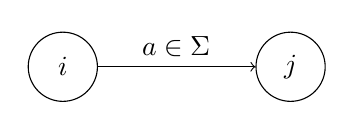
\begin{tikzpicture}[node distance=2cm]
        \node[state] (i) {\(i\)};
        \node[state] (j) [right=of i] {\(j\)};
        
        \path[->] (i) edge [above] node {\(a \in \Sigma\)} (j);
    \end{tikzpicture}
    \caption*{Altfel: \(R_{i, i}^{0} = \Set{ a \in \Sigma | \delta'(i, a) = i } \cup \Set{ \lambda }\)}
    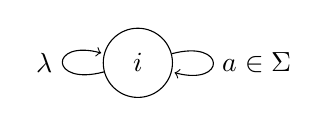
\begin{tikzpicture}
        \node[state] (i) {\(i\)};
        
        \path[->] (i)
            edge [loop right] node {\(a \in \Sigma\)} ()
            edge [loop left] node {\(\lambda\)} ();
    \end{tikzpicture}
\end{figure}

\medskip

\textbf{Ipoteza de inducție.} Pentru \(k \geq 1\), presupunem că știm deja cât este
\(R_{i, j}^{k - 1}\), \(\forall i, j \in \overline{1, n}\).
Vrem să scriem \(R_{i, j}^{k}\) în funcție de câteva \(R^{k - 1}\).

Pentru a determina toate drumurile de la \(i\) la \(j\) care trec prin stări cu indice cel mult \(k\), putem începe mai întâi cu toate drumurile \(R_{i, j}^{k - 1}\), deoarece \(k - 1 \leq k\).
La acestea se adaugă toate drumurile de la \(i\) la \(j\) care trec și prin starea intermediară \(k\).

\begin{figure}[!h]
    \centering
    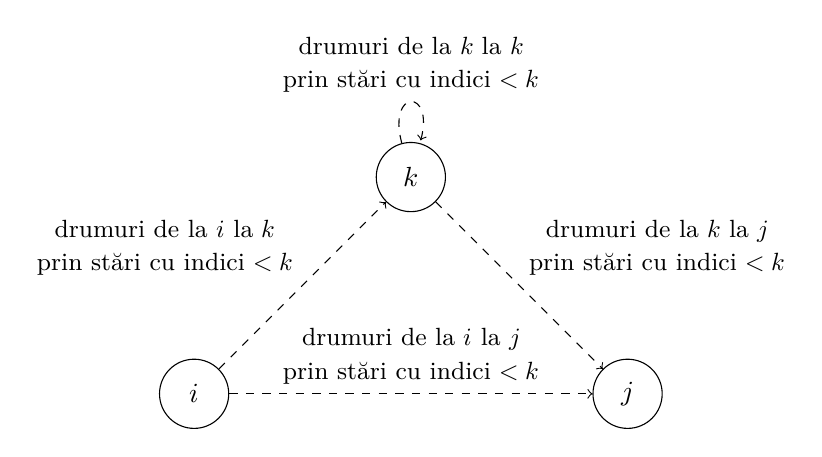
\begin{tikzpicture}[auto, node distance=3cm]
        \node[state] (i) {\(i\)};
        \node[state] (k) [above right=of i] {\(k\)};
        \node[state] (j) [below right=of k] {\(j\)};
        
        \path[dashed, ->] (i)
            edge node [align=center] {\small drumuri de la \(i\) la \(k\) \\ \small prin stări cu indici \(< k\)} (k)
            edge node [align=center] {\small drumuri de la \(i\) la \(j\) \\ \small prin stări cu indici \(< k\)} (j);
        \path[dashed, ->] (k)
            edge [loop above] node [align=center] {\small drumuri de la \(k\) la \(k\) \\ \small prin stări cu indici \(< k\)} ()
            edge node [align=center] {\small drumuri de la \(k\) la \(j\) \\ \small prin stări cu indici \(< k\)} (j);
    \end{tikzpicture}
    \caption*{\(
        R_{i, j}^{k} = R_{i, j}^{k - 1} \cup (R_{i, k}^{k - 1} \cdot (R_{k, k}^{k - 1})^* \cdot R_{k, j}^{k - 1})
    \)}
\end{figure}

\clearpage

Acum putem demonstra mult mai ușor că pentru orice mulțime de cuvinte \(R_{i, j}^{k}\) există o expresie regulată \(r_{i, j}^{k}\) astfel încât \(L(r_{i, j}^{k}) = R_{i, j}^{k}\).
\begin{proof}
Demonstrăm prin inducție după \(k\).

\medskip

\textbf{Cazul de bază.} Când \(k = 0\), \(R_{i, j}^{0}\) este o mulțime finită formată din toate literele
pentru care există tranziții de la \(i\) la \(j\), și eventual \(\lambda\) dacă \(i = j\).

\(r_{i, j}^{0}\) poate fi scris ca o disjuncție între aceste litere.

\medskip

\textbf{Ipoteza de inducție.} Presupunem că pentru orice \(R_{i, j}^{k}\) putem construi o expresie regulată \(r_{i, j}^{k}\) cu \(L(r_{i, j}^{k}) = R_{i, j}^{k}\).

\smallskip

Definim \(r_{i, j}^{k + 1} = r_{i, j}^{k} \cup (r_{i, k + 1}^{k} (r_{k + 1, k + 1}^{k})^{*} r_{k + 1, j}^{k})\).

Arătăm că această expresie regulată într-adevăr corespunde lui \(R_{i, j}^{k + 1}\):
\begin{align*}
L(r_{i, j}^{k + 1}) &= L((r_{i, j}^{k} \cup (r_{i, k + 1}^{k} (r_{k + 1, k + 1}^{k})^{*} r_{k + 1, j}^{k})) && \text{definiția lui \(r_{i, j}^{k + 1}\)} \\
&= L(r_{i, j}^{k}) \cup (L(r_{i, k + 1}^{k}) (L(r_{k + 1, k + 1}^{k}))^{*} L(r_{k + 1, j}^{k})) \\
&= R_{i, j}^{k} \cup (R_{i, k + 1}^{k} (R_{k + 1, k + 1}^{k})^{*} R_{k + 1, j}^{k}) && \text{ipoteza de inducție} \\
&= R_{i, j}^{k + 1} && \text{definiția lui \(R_{i, j}^{k + 1}\)}
\end{align*}
\end{proof}

Un cuvânt este acceptat de DFA dacă este acceptat:
\begin{itemize}
    \item de expresia pentru cuvintele care merg din starea inițială în prima stare finală (\(r_{1, f_1}^{n}\))
    \item \emph{sau} de expresia pentru cuvintele care merg din starea inițială în a doua stare finală (\(r_{1, f_2}^{n}\))
    \item etc.
\end{itemize}

Expresia finală pentru tot DFA-ul este:
\[
E = r_{1, f_1}^{n} \cup r_{1, f_2}^{n} \cup \dots \cup r_{1, f_{|F|}}^{n} = \bigcup\limits_{f \in F'} r_{1, f}^{n}
\]

\end{document}
